\documentclass{ximera}

\outcome{Compare and contrast the Intermediate Value Theorem, Mean Value Theorem, and Rolle's Theorem.}
\outcome{What does the MVT tell us?}
\outcome{What important calculus ideas are consequences of the MVT?}
\outcome{Determine whether Rolle's Theorem and/or MVT can be applied.}
\outcome{Find the values guaranteed by Rolle's Theorem or MVT.}
\outcome{Use MVT to solve word problems.}

\title{Mean value theorem}

\begin{document}

\begin{abstract}
  The mean value theorem relates the derivative of the function to the
  average growth rate.
\end{abstract}
\maketitle

Here are some  interesting questions involving derivatives:

\begin{enumerate}
\item Suppose you toss a ball into the air and then catch it. Must the
  ball's vertical velocity have been zero at some point?
\item Suppose you drive a car from toll booth on a toll road to
  another toll booth $30$ miles away in half of an hour. Must you have
  been driving at $60$ miles per hour at some point?
\item Suppose two different functions have the same derivative. What
  can you say about the relationship between the two functions?
\end{enumerate}

While these problems sound very different, it turns out that the
problems are very closely related. We'll start simply:

\begin{theorem}[Rolle's Theorem]
Suppose that $f(x)$ is differentiable on the interval $(a,b)$, is
continuous on the interval $[a,b]$, and $f(a)=f(b)$. Then
\[
f'(c)=0
\]
for some $a<c<b$.
\end{theorem}
\begin{image}
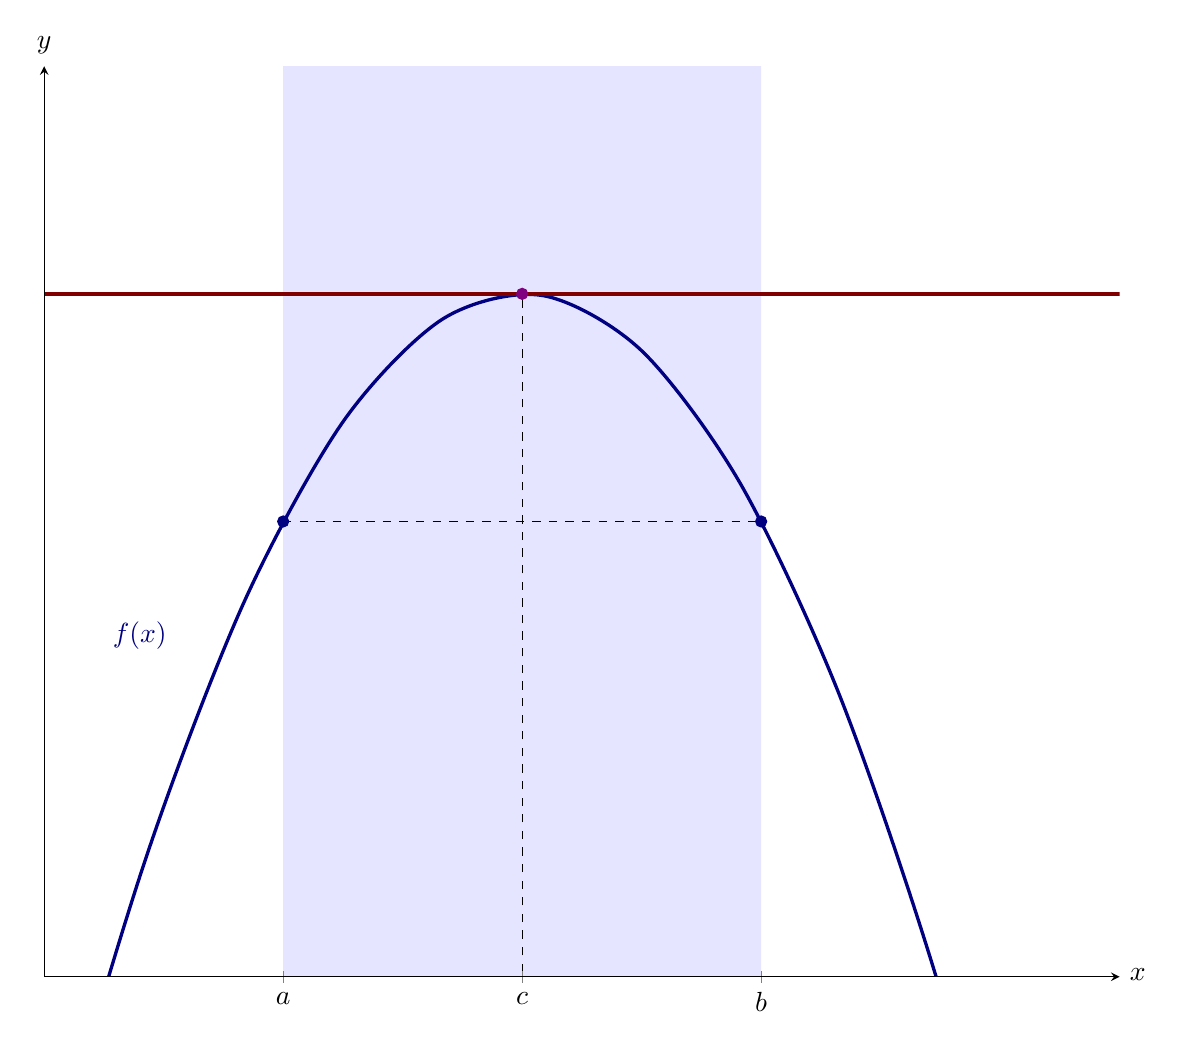
\begin{tikzpicture}
\colorlet{penColor}{blue!50!black} % Color of a curve in a plot
\colorlet{penColor2}{red!50!black} % Color of a curve in a plot
\colorlet{fill2}{blue!10} % Color of fill in a plot
\colorlet{penColor3}{red!50!blue} % Color of a curve in a plot
	\begin{axis}[
            xmin=0, xmax=4.5,ymin=1,ymax=5,
            width=6in,
            axis lines =left, xlabel=$x$, ylabel=$y$,
            every axis y label/.style={at=(current axis.above origin),anchor=south},
            every axis x label/.style={at=(current axis.right of origin),anchor=west},
            xtick={1,2,3}, xticklabels={$a$,$c$,$b$},
            ytickmin=1, ytickmax=0,
            axis on top,
          ]       
          \addplot [draw=none, fill=fill2,domain=(1:3)] {5} \closedcycle;       
	  \addplot [very thick,penColor, smooth] {-(x-2)^2+4};
          \addplot [very thick,penColor2, smooth] {4};
          \node at (axis cs:.4,2.5) [penColor] {$f(x)$}; 
          \addplot [black,dashed] plot coordinates {(2,0) (2,4)};
          \addplot [black,dashed] plot coordinates {(1,3) (3,3)};
          \addplot[color=penColor3,fill=penColor3,only marks,mark=*] coordinates{(2,4)};  %% closed hole          
          \addplot[color=penColor,fill=penColor,only marks,mark=*] coordinates{(1,3)};  %% closed hole          
          \addplot[color=penColor,fill=penColor,only marks,mark=*] coordinates{(3,3)};  %% closed hole          
        \end{axis}
\end{tikzpicture}
\end{image}


\begin{question}
  Suppose you toss a ball into the air and then catch it. Must the
  ball's vertical velocity have been zero at some point?
  \begin{multipleChoice}
    \choice[correct]{Yes.}
    \choice{No.}
    \choice{There is no way to tell.}
  \end{multipleChoice}  
\end{question}


Rolle's Theorem is a special case of a more general theorem.

\begin{theorem}[Mean Value Theorem]
Suppose that $f(x)$ has a derivative on the interval $(a,b)$ and is
continuous on the interval $[a,b]$.  Then
\[
f'(c)=\frac{f(b)-f(a)}{b-a}
\]
for some $a<c<b$. 
\end{theorem}

\begin{image}
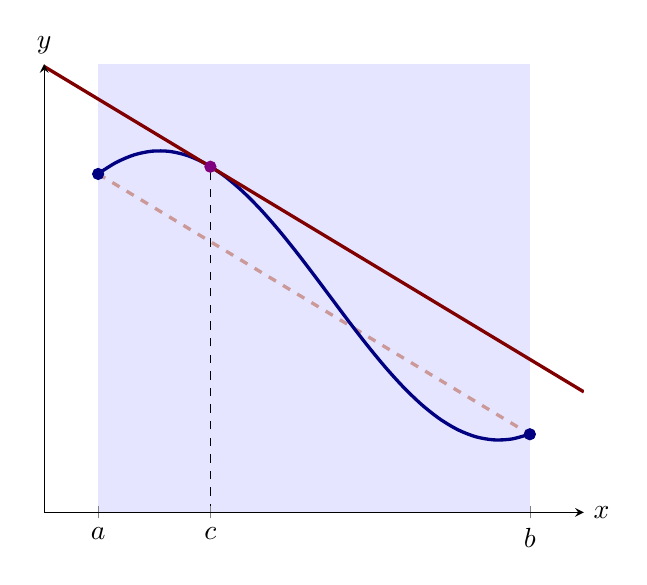
\begin{tikzpicture}
\colorlet{penColor}{blue!50!black} % Color of a curve in a plot
\colorlet{penColor2}{red!50!black} % Color of a curve in a plot
\colorlet{fill2}{blue!10} % Color of fill in a plot
\colorlet{penColor3}{red!50!blue} % Color of a curve in a plot
	\begin{axis}[
            xmin=.5, xmax=5.5,ymin=0,ymax=3.1,
            axis lines =center, xlabel=$x$, ylabel=$y$,
            every axis y label/.style={at=(current axis.above origin),anchor=south},
            every axis x label/.style={at=(current axis.right of origin),anchor=west},
            xtick={1,2.04,5}, xticklabels={$a$,$c$,$b$},
            ytickmin=1, ytickmax=0,
            axis on top,
          ] 
          \addplot [draw=none, fill=fill2,domain=(1:5)] {3.1} \closedcycle;       
          \addplot [penColor2!40!white,very thick,dashed] plot coordinates {(1,.84+1.5) (5,1.5-.96)};        
          \addplot [black,dashed] plot coordinates {(2.04,0) (2.04,1.5+.89)};        
	  \addplot [very thick,penColor, smooth,domain=(1:5)] {sin(deg(x))+1.5};
          \addplot [very thick,penColor2,domain=(.5:5.5)] {-.45*(x-2.04)+.89+1.5};
          %\node at (axis cs:.4,2.5) [penColor] {$f(x)$}; 
          \addplot[color=penColor,fill=penColor,only marks,mark=*] coordinates{(1,.84+1.5)};  %% closed hole          
          \addplot[color=penColor,fill=penColor,only marks,mark=*] coordinates{(5,-.96+1.5)};  %% closed hole          
          \addplot[color=penColor3,fill=penColor3,only marks,mark=*] coordinates{(2.04,.89+1.5)};  %% closed hole          
        \end{axis}
\end{tikzpicture}
\end{image}

\begin{question}
  Suppose you drive a car from toll booth on a toll road to another
  toll booth $30$ miles away in half of an hour. Must you have been
  driving at $60$ miles per hour at some point?
  \begin{multipleChoice}
    \choice[correct]{Yes.}
    \choice{No.}
    \choice{There is no way to tell.}
  \end{multipleChoice}  
\end{question}


\begin{question} Let $f(x) = x^2$.
  Find a value $c\in (-1,2)$ so that $f'(c)$ equals the slope between
  the endpoints of $f(x)$ on $[-1,2]$.  $c=$\answer{1/2}
\end{question}

\begin{question}
Verify that $f(x) = x/(x+2)$ satisfies the hypotheses of the Mean
Value Theorem on the interval $[1,4]$ and then find all of the values,
$c$, that satisfy the conclusion of the theorem.
$c=$\answer{sqrt(18)-2}
\end{question}

\begin{question}
Write down at least \textbf{five} questions for this lecture. After
you have your questions, label them as ``Level 1,'' ``Level 2,'' or
``Level 3'' where:
\begin{description}
\item[Level 1] Means you know the answer, or know exactly how to do this problem.
\item[Level 2] Means you think you know how to do the problem, or will soon learn how to do the problem.
\item[Level 3] Means you have no idea how to do the problem. 
\end{description}
  \begin{freeResponse}
  \end{freeResponse}
\end{question}

\end{document}
